\section{Implementacja systemu na poziomie klas}
Oprogramowanie podzielono na sześć klas: \emph{App}, \emph{VideoCapture}, \emph{YoloInferenceConfig}, \emph{ImageProcessor}, \emph{VideoProcessingEngine} oraz \emph{GUI}.

\emph{App} jest punktem centralnym aplikacji. W tym miejscu rozpoczyna się program oraz tworzone są instancje pozostałych pięciu klas. Pierwszym zadaniem klasy jest utworzenie obiektów pozostałych klas. Następnie klasa ta służy jako interfejs do komunikacji między modułem interfejsu graficznego użytkownika (\emph{GUI}) a sekcją logiczną — w tym do pobrania informacji o liście dostępnych kamer (\emph{VideoCapture}), ustawienia parametrów inferencji detektora (\emph{ImageProcessor}) oraz do komunikacji z silnikiem przetwarzania wideo (\emph{VideoProcessingEngine}). Ponadto klasa ta implementuje metodę, która uruchamia alarm dźwiękowy (\emph{play\_audio\_alert}).
 
\emph{VideoCapture} służy do obsługi źródła wideo. Klasa dostarcza kluczową metodę, \emph{get\_frame}, której wywołanie zwraca informację o tym, czy źródło wideo nadal jest dostępne oraz najnowszą dostępną klatkę z kamery. Ponadto warto wyróżnić metodę do pozyskiwania dostępnych kamer (\emph{get\_available\_sources}). Klasa ta zawiera również metody \emph{start\_capture} oraz \emph{end\_capture}, odpowiedzialne kolejno za ustanowienie połączenia z podaną jako argument kamerą oraz za zwolnienie tego połączenia.

\emph{YoloInferenceConfig} to klasa, której głównym celem jest przechowywanie parametrów inferencji (progu ufności oraz wykrywanych klas) oraz dostarczenie metod do zmiany tych parametrów. Klasę utworzono w celu zachowania większej czytelności kodu w \emph{ImageProcessor}, dlatego też jest ona dziedziczona przez \emph{ImageProcessor}. W chwili uruchomienia aplikacji klasa jest inicjalizowana domyślnymi parametrami: próg ufności równy $0.5$ oraz \emph{człowiek} jako wykrywana klasa.

\emph{ImageProcessor} służy do przetwarzania oraz analizy obrazu. Kluczowe trzy metody to: \emph{detect\_objects}, zwracająca liczbę wykrytych obiektów oraz wyniki detekcji na podstawie podanej klatki obrazu; \emph{visualize\_objects\_presence}, która na podstawie w.w. wyników detekcji rysuje prostokąty ograniczające wykryte obiekty; \emph{fit\_frame\_into\_screen}, która zmniejsza rozmiar podanej klatki, jeżeli jest większa niż rozmiar ekranu monitora podłączonego do komputera.

\emph{VideoProcessingEngine} stworzono w celu koordynacji i rozplanowania wszystkich zadań koniecznych do uzyskania kolejnych klatek obrazu, gotowych do wyświetlenia w graficznym interfejsie użytkownika, oraz realizacji celu alarmowania dźwiękowego użytkownika, kiedy jest to konieczne. Zbiór zadań obejmuje pobranie klatki z kamery, detekcję obiektów, przetworzenie klatki w celu wizualizacji obiektów, alarmowanie dźwiękowe użytkownika oraz umieszczenie klatki w buforze wyjściowym. Zadania te nie mają implementacji w samej klasie i są realizowane za pomocą metod wywoływanych z innych klas (\emph{App}, \emph{ImageProcessor} oraz \emph{VideoCapture}).
Podsumowując tę część opisu, jest to klasa realizująca moduł silnika przetwarzania wideo opisanego w rozdziale \ref{chap:architektura}. Klasa ta dostarcza również metody umożliwiające wznowienie (\emph{set\_video\_source}) lub zatrzymanie (\emph{remove\_video\_source}) kolejnych wykonań sekwencji opisanych w ww. rozdziale, wywołując przy tym odpowiednio metody \emph{VideoCapture}: \emph{start\_capture} oraz \emph{end\_capture}.

\emph{GUI} to graficzny interfejs użytkownika aplikacji. Składa się on z wyświetlacza klatek obrazu oraz panelu sterowania. Jak wcześniej wspomniano, wykorzystuje on klasę \emph{App} do komunikacji z resztą systemu. Dotyczy to zarówno komunikacji dwustronnej z \emph{ImageProcessor}, służącej do pobrania parametrów detektora oraz ich ustawienia w panelu sterowania, jak i komunikacji dwustronnej z \emph{VideoProcessingEngine} w celu pobrania klatki z bufora wyjściowego oraz kontroli sekwencji przetwarzania. Ponadto interfejs komunikuje się jednostronnie z \emph{VideoCapture}, aby uzyskać listę dostępnych kamer.

Opisane zależności komunikacyjne między klasami, w tym typy połączeń między nimi (kompozycja, agregacja, dziedziczenie), zilustrowano uproszczonym diagramem UML na rysunku \ref{fig:uprosczony-diagram-klas}. 
%Pełen diagram UML przedstawiono na rysunku \ref{fig:diagram-klas}. 

\begin{figure}[H]
    \centering
    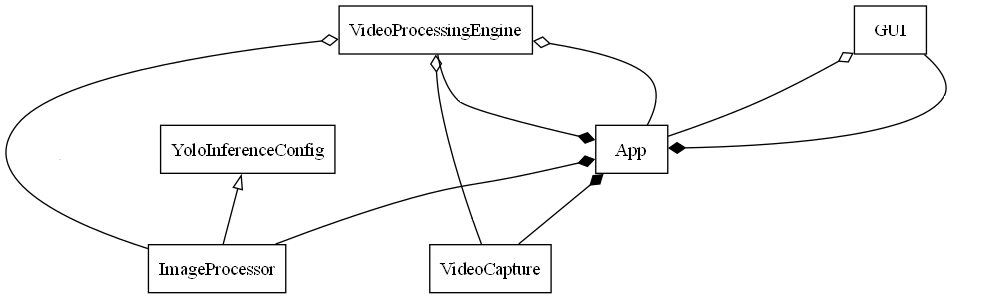
\includegraphics[width=\linewidth]{r_implementacja/klasy/simplified_classes.png}
    \caption{Uprosczony diagram klas UML (bez metod i pól) wygenerowany przez bilbiotekę \emph{pylint}.}
    \label{fig:uprosczony-diagram-klas}
\end{figure}

Tak jak wspomniano, klasa \emph{YoloInferenceConfig} nie jest instancjowana – programowe użycie jej pól odbywa się wewnątrz \emph{ImageProcessor}, a jej metody są wywoływane za pośrednictwem obiektu klasy \emph{ImageProcessor}. Umożliwia to dziedziczenie \emph{YoloInferenceConfig} przez \emph{ImageProcessor}.

\emph{App}, jako punkt startowy aplikacji, tworzy w swoim konstruktorze obiekty klas \emph{VideoCapture}, \emph{ImageProcessor}, \emph{VideoProcessingEngine} oraz \emph{GUI}. Istnienie tych obiektów jest zależne od istnienia klasy \emph{App} – z perspektywy UML jest to kompozycja. Nazwy tych obiektów to, według kolejności: \emph{\_image\_processor}, \emph{\_video\_capture}, \emph{\_video\_processing\_engine} oraz \emph{\_gui}. Następnie plik główny programu (\emph{main.py}) wywołuje metodę \emph{run}. Metoda ta uruchamia silnik generacji klatek (\emph{self.\_video\_processing\_engine.run()}) oraz wyświetla graficzny interfejs użytkownika (\emph{self.\_gui.show()}). Po zamknięciu GUI wykonywana jest ostatnia instrukcja, wyłączająca silnik generacji klatek (\emph{self.\_video\_processing\_engine.shutdown()}). Opisane użycie zaprezentowano fragmentem kodu w listingu \ref{lst:app-instancjowanie}.

\begin{lstlisting}[caption={Tworzenie obiektów klas wewnątrz \emph{App} oraz uruchomienie w niej różnych sekcji aplikacji.}, label={lst:app-instancjowanie}]
class App:
    # Konstruktor App
    def __init__(self) -> None:
        # ... reszta kodu
        # Tworzenie obiektow klas:
        self._video_capture = VideoCapture()
        self._image_processor = ImageProcessor()
        self._video_processing_engine = VideoProcessingEngine(self._video_capture, self._image_processor, self)
        self._gui = GUI(self)
        # reszta kodu ...

    # Metoda uruchamiajaca poszczegolne sekcje aplikacji
    def run(self) -> None:
        self._video_processing_engine.run()
        self._gui.show()
        self._video_processing_engine.shutdown()
\end{lstlisting}

Tak jak wspomniano w opisach klas, \emph{App} jest interfejsem komunikacyjnym między \emph{GUI} a resztą klas potrzebnych \emph{GUI}. Do \emph{GUI} przekazywana jest referencja (obiekt) \emph{App}, z której poziomu utworzono obiekt \emph{GUI}. W celu pobrania bądź zmiany informacji w innych modułach, \emph{GUI} wywołuje metody \emph{App} poprzez tę referencję. Z perspektywy \emph{GUI} jest to agregacja. Taki sam typ relacji dotyczy również \emph{VideoProcessingEngine} względem \emph{App}, której referencję \emph{VideoProcessingEngine} wykorzystuje do wywołania metody alarmującej dźwiękowo użytkownika. Agregacja w \emph{VideoProcessingEngine} występuje także względem \emph{ImageProcessor} oraz \emph{VideoCapture}.

